\subsection{Comparison of Fit vs Non-Fit}

The method proposed by P. Hudzovic is compared  to  itself  with  and  without a
least squared fit of the parameters $T$ and  $r$. Similarly, the method proposed
by  L.  Sani is also compared to itself with and without a least squared fit  of
$T$ and $r$.

The input curve in Sani's case  was  a 4th order Hudzovic transfer function with
$r=\frac{1}{6}$ and $T=1$.  The  input  curve in Hudzovic's case was a 4th order
Sani transfer function with $r=0.5$  and  $T=1$.

The reason for choosing an ``unsuitable'' input curve was to  make it impossible
for the method  under  test  to  calculate a perfectly correct transfer function
such that the error would be 0.

The test was performed twice for  each method, once with no input noise and once
with  random noise (20\% normalised amplitude) modulated onto the input  signal.

\begin{figure}[t]
    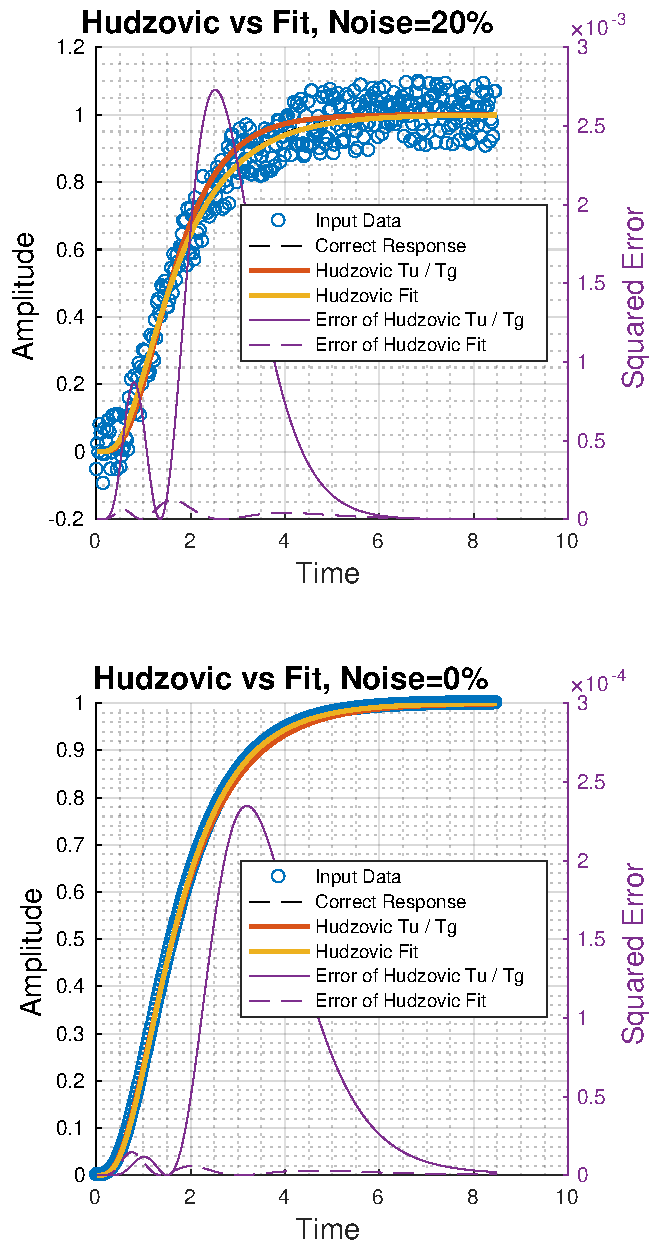
\includegraphics[width=\linewidth]{images/hudzovic_vs_fit}
    \caption{Comparison of a normal Hudzovic Tu/Tg lookup to a least square refinement. Order n=4, Noise=20\% and 0\%}
    \label{fig:hudzovic_vs_fit}
\end{figure}

\begin{figure}[t]
    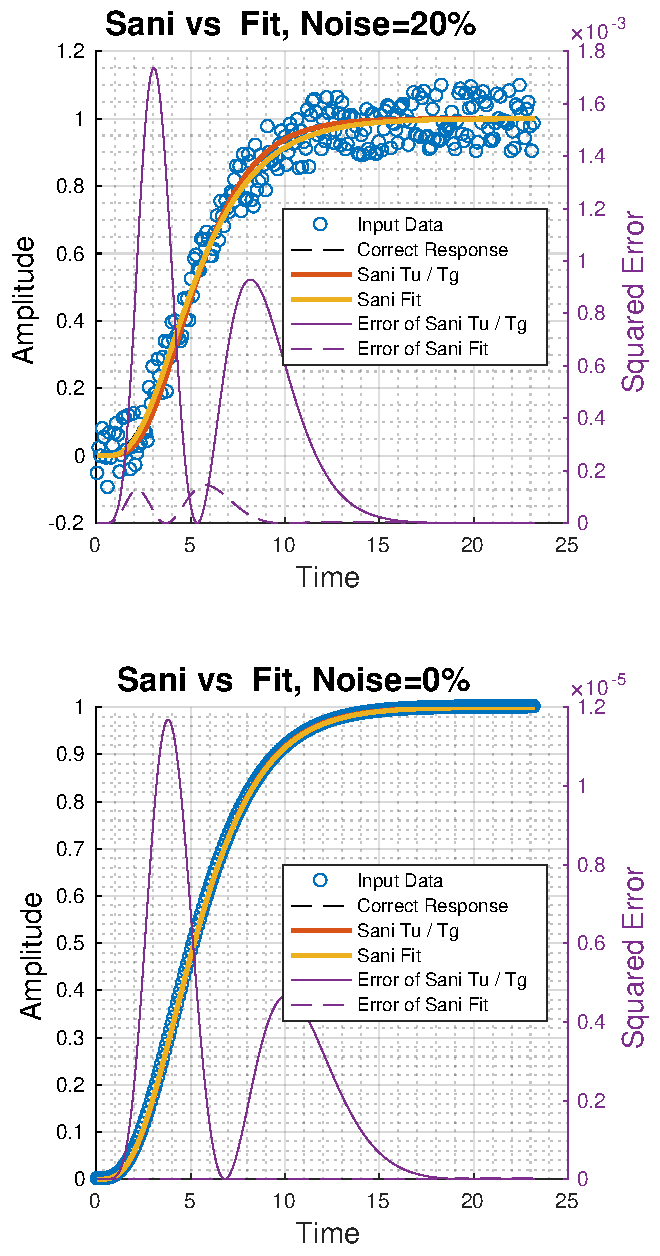
\includegraphics[width=\linewidth]{images/sani_vs_fit}
    \caption{Comparison of a normal Sani Tu/Tg lookup to a least square refinement. Order n=4, Noise=20\% and 0\%}
    \label{fig:sani_vs_fit}
\end{figure}

The   results   can   be   seen   in   figures   \ref{fig:hudzovic_vs_fit}   and
\ref{fig:sani_vs_fit}. The blue circles show the raw  input  data  to the method
under test. The red  curve  shows  the  step  response of the resulting transfer
function \textit{without} fitting and the yellow curve  shows  the step response
\textit{with} a least squares fit.

Further, the two purple  curves  on  a  second  Y  axis show the \textit{squared
error}  of the output function to the original non-noisy input function of  each
data point. The dashed purple line is the error of the fitted result whereas the
continuous purple line is the error of the non-fitted result.

It is fairly clear that in all  four  cases  the  least  square  fit yields more
accurate results. The maximum squared error of the non-fitted methods (with 20\%
input  noise)  is  around $2x10^{-3}$, whereas the maximum squared error of  the
fitted  methods  is  around  $1x10^{-4}$. This leads to an improvement factor of
about 5.
